\chapter{Resultados}

\section{Evaluación de nuestra implementación}

En este momento vamos a evaluar debilidades y fortalezas de nuestra implementación de ext2. 

La debilidad obvia, y que no nos importa, es que la implementación no es completa: carece de manejo de permisos de archivos, cosa que no nos importa en DeliriOS.

Además, es mucho más simple que la implementación de ext2 de otros sistemas operativos como Linux, y usa algoritmos mucho menos sofisticados. Sin embargo, no esperaremos que su performance sea mucho peor. Esto lo veremos más adelante.

Una métrica no siempre utilizada al comparar varias implementaciones de una misma especificación es su simplicidad. Aquí sí lo haremos, dado que DeliriOS es un sistema operativo que se concentra en ser minimal, aunque funcional.

Comparemos la cantidad de líneas de código de cada implementación.

\begin{figure}
  \centering
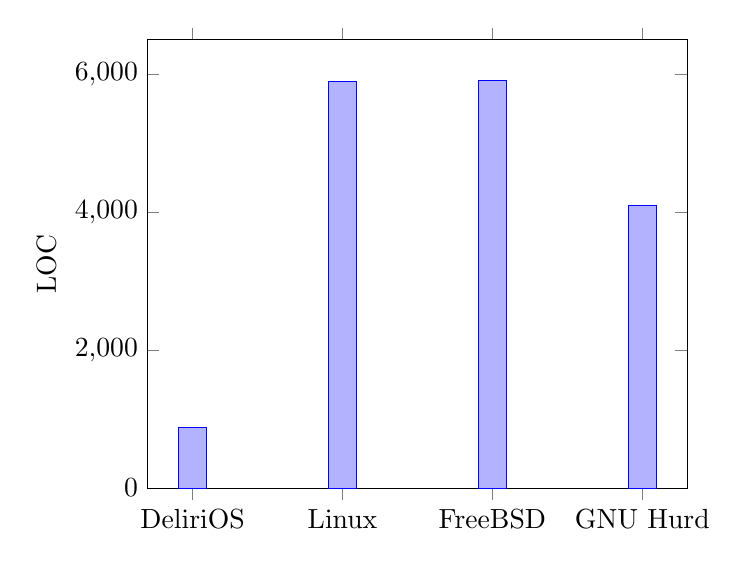
\begin{tikzpicture}
\begin{axis}[
	%x tick label style={/pgf/number format/1000 sep=},
  symbolic x coords={DeliriOS, Linux, FreeBSD, GNU Hurd},
	ylabel=LOC,
  xtick=data,
  ymin=0,
	ybar,
]
\addplot 
	coordinates {
    (DeliriOS,876)
    (Linux,5899)
    (FreeBSD,5910)
    (GNU Hurd,4104)};
\end{axis}
\end{tikzpicture}
\caption{Líneas de código de la implementación de ext2 de cada sistema operativo. El programa cloc fue utilizado para medirlas, dado que cuenta las lineas de código puro, sin contar líneas vacías y de comentarios.}
\end{figure}

\begin{figure}
  \centering
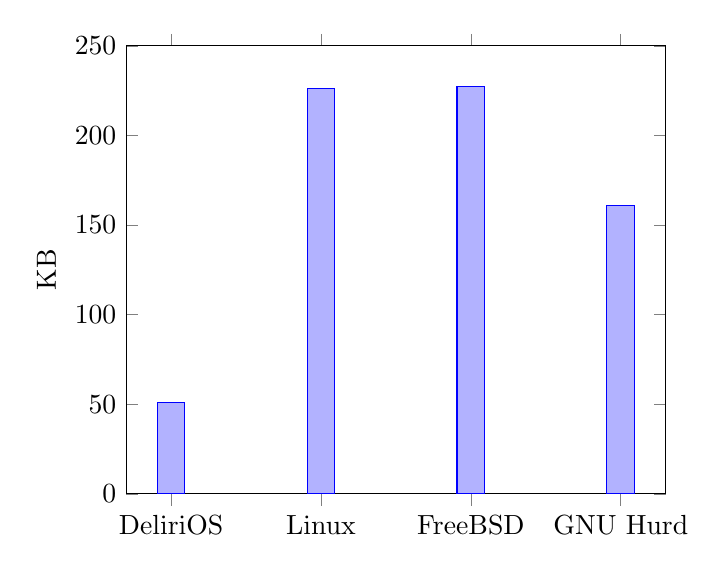
\begin{tikzpicture}
\begin{axis}[
	%x tick label style={/pgf/number format/1000 sep=},
  symbolic x coords={DeliriOS, Linux, FreeBSD, GNU Hurd},
	ylabel=KB,
  xtick=data, 
  ymin=0,
	ybar,
]

%(DeliriOS,52477)
%(Linux,231427)
%(FreeBSD,232832)
%(GNUHurd,164757)};
\addplot 
	coordinates {
    (DeliriOS,51.24)
    (Linux,226.00)
    (FreeBSD,227.37)
    (GNU Hurd,160.89)};
\end{axis}
\end{tikzpicture}
\caption{Tamaño del código fuente de la implementación de ext2 de cada sistema operativo.}
\end{figure}


Como puede verse, la implementación de DeliriOS es realmente simple y corta. Esto es muy bueno, dado que por un lado es más fácil de entender para alguien que se acople al proyecto, y por otro lado permite que el binario de DeliriOS siga siendo diminuto (entra entero en la cache L1 de código de un core de un procesador moderno).



\section{Performance de nuestra implementación}

\begin{enumerate}
  \item Tomar tiempos.
\end{enumerate}

